\chapter{Integra UFF - Especificação de Requisitos do Software}
\thispagestyle{empty} % retira numeracao da pagina, conforme as normas de apresentacao.

Este capítulo apresenta a especificação de software do Integra UFF. Aqui serão descritos os objetivos, ambientes, suposições, requisitos e interfaces pensadas durante o desenvolvimento da mesma. Assim como as funcionalidades e telas implementadas no produto final. 

\section{Descrição Geral}

\subsection{Perspectiva do produto}

O produto implementa uma interface que agrega conteúdos obtidos de outros sistemas LMSs já existentes estendendo suas funcionalidades. Ele consiste de uma aplicação móvel cliente e uma aplicação web remota que acessa as interfaces públicas dos sistemas terceiros. A aplicação web oferece uma \textit{Application programming interface} (API) que atende os pedidos da aplicação móvel, intermediando o acesso aos sistemas externos.
A aplicação web contará com uma base de dados auxiliar, para controle dos usuários e comunicação instantânea.

\subsection{Funções do Produto}

A aplicação deve ser capaz permitir a autenticação do usuário nos sistemas integrados, obtendo o conteúdo necessário para fornecer as principais funcionalidades contempladas para o Integra UFF, que são:

\begin{itemize}
    \item Disponibilização de uma listagem das disciplinas do usuário.
    \item Tópicos (Grupo de Discussão).
    \item Listagem e \textit{download} de Arquivos.
    \item Calendário de Eventos das Disciplinas.
    \item Envio de Mensagens.
    \item Lista de Amigos.
\end{itemize}

\subsection{Classes de Usuário e Caracterísiticas}

As classes de usuários previstas serão, o aluno participante da disciplina, o professor da disciplina no papel de moderador do grupo, e os administradores do sistema que exercerão funções de manutenção do sistema. 

\subsection{Ambiente Operacional}

A interface do usuário será executada em dispositivos móveis como \textit{smartphones} e \textit{tablets}, nos três sistemas operacionais mais utilizados, sendo eles o iOS da fabricante \textit{Apple}, o \textit{Android} da \textit{Google} e o \textit{Windows Phone} 8 da \textit{Microsoft}.
A aplicação remota será executada em uma máquina servidora com sistema operacional Linux, distribuição Ubuntu, com servidor \textit{web} Apache ou Nginx com o módulo \textit{passenger-phusion} devidamente configurado para servir aplicações \textit{Ruby on Rails}, todos em suas versões mais recentes.

\subsection{Restrições de \textit{Design} e Implementação}
Por se tratar de um trabalho acadêmico,  não haverão restrições de \textit{design} e implementação rígidas, deixando os desenvolvedores juntamente ao orientador livres para escolher as tecnologias verificadas e tidas como adequadas para a solução. No entanto toda a integração feita com os sistemas LMSs são limitadas a disponibilidade de uma API acessível pela \textit{web} e ao conteúdo fornecido por elas. 

\subsection{Suposições e Dependências}

O sistema tem como dependências a plataforma de desenvolvimento móvel \textit{Apache Cordova}, o \textit{framework} de desenvolvimento ágil \textit{Rails}, o \textit{framework} AngularJS, o \textit{framework} de CSS \textit{Twitter Bootstrap} e outros \textit{plugins} indentificados no decorrer do desenvolvimento.

\section{Requisitos de Interface Externa}

\subsection{Interfaces de Usuário}
As interfaces de usuário serão desenvolvidas com as tecnologias e padrões abertos \textit{web}, \textit{Javascript}, CSS3 e HTML5 e serão responsivas, se ajustando a diversos tipos de dispositivos e tamanhos de tela.

\subsection{Interfaces de Hardware}

O \textit{software} será executado em dispositivos móveis, \textit{smartphones} e \textit{tablets}, do tipo \textit{Android}, \textit{Windows} e \textit{iPhone} que se comunicará com os serviços de uma aplicação intermediária, executada em um computador servidor \textit{web}, que por sua vez se comunica com as APIs das diversas plataformas de ensino integradas.

\subsection{Interfaces de Software}

O \textit{software} executado no dispositivo móvel, utiliza o empasulamento de uma aplicação \textit{web} para as diversas plataformas móveis através do \textit{framework} \textit{phonegap}, de forma totalmente transparente ao usuário que utiliza o \textit{software} como um aplicativo nativo. Esta \textit{webapp} se comunica com a aplicação servidora intermediária através de recursos \textit{web} executados no \textit{software} Apache ou \textit{Ngnx} com o \textit{framework} \textit{Rails}. A aplicação intermediária por sua vez utiliza as intefaces disponibilizadas pelas plataformas de ensino, que podem ser diversas e implementadas sob a forma de \textit{plugins}.

\subsection{Interfaces de Comunicação}

A comunicação é totalmente via \textit{web}, utilizando o protocolo HTTP entre a aplicação cliente, a aplicação servidor e as APIs das plataformas de ensino, seguindo o estilo arqutetural REST entre a a aplicação cliente e a camada intermediária.

\section{Funcionalidades do Sistema}

Nesta seção descreveremos as funcionalidades implementadas na versão final do aplicativo Integra UFF, assim como suas telas.

\subsection{Sincronizar com uma plataforma}

O primeiro passo para começar a utilizar o Integra UFF é realizar a sincronização com uma das plataformas integradas. Atualmente apenas o Conexão UFF está disponível. 

Ao acessar o aplicativo o usuário verá uma tela com um botão de sincronização, que ao apertado exibirá um formulário de autenticação, figura \ref{sincronizacao}. Feito a autenticação, o usuário será redirecionado para o menu principal do aplicativo, figura \ref{menuprincipal}, com o acesso a Disciplinas, Eventos e Arquivos. 

O caso de uso da sincronização está explicitado na tabela \ref{table:sincronizacao}.

\begin{figure}[H]
    \centering
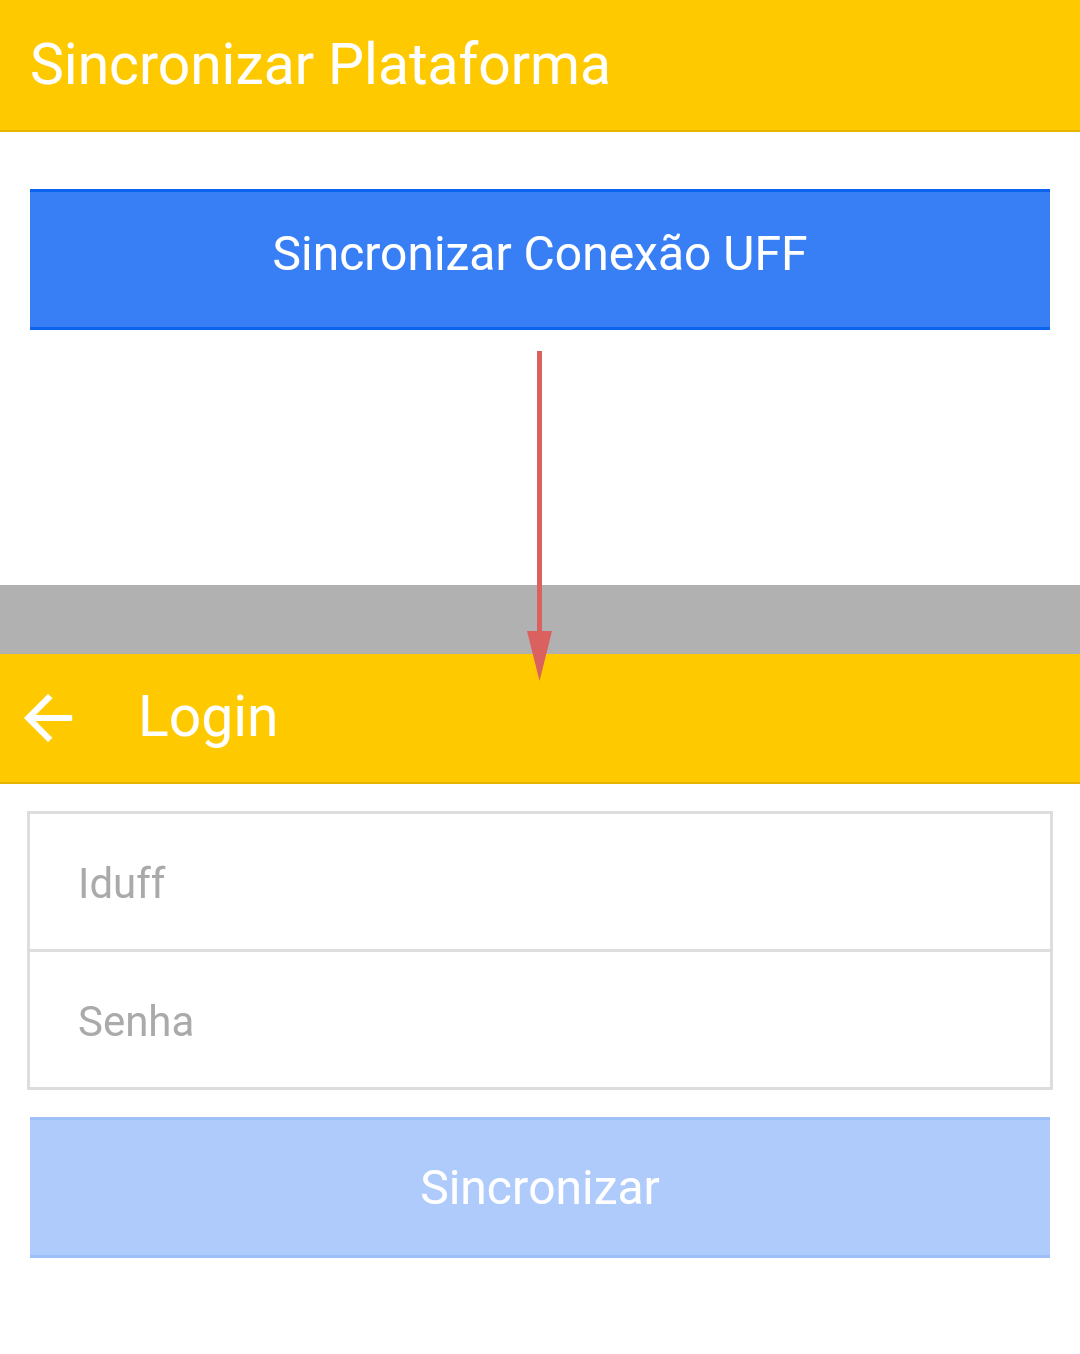
\includegraphics[scale=0.15]{sincronizacao}
    \caption{Autenticação na plataforma}
    \label{sincronizacao}
\end{figure}

\begin{figure}[H]
    \centering
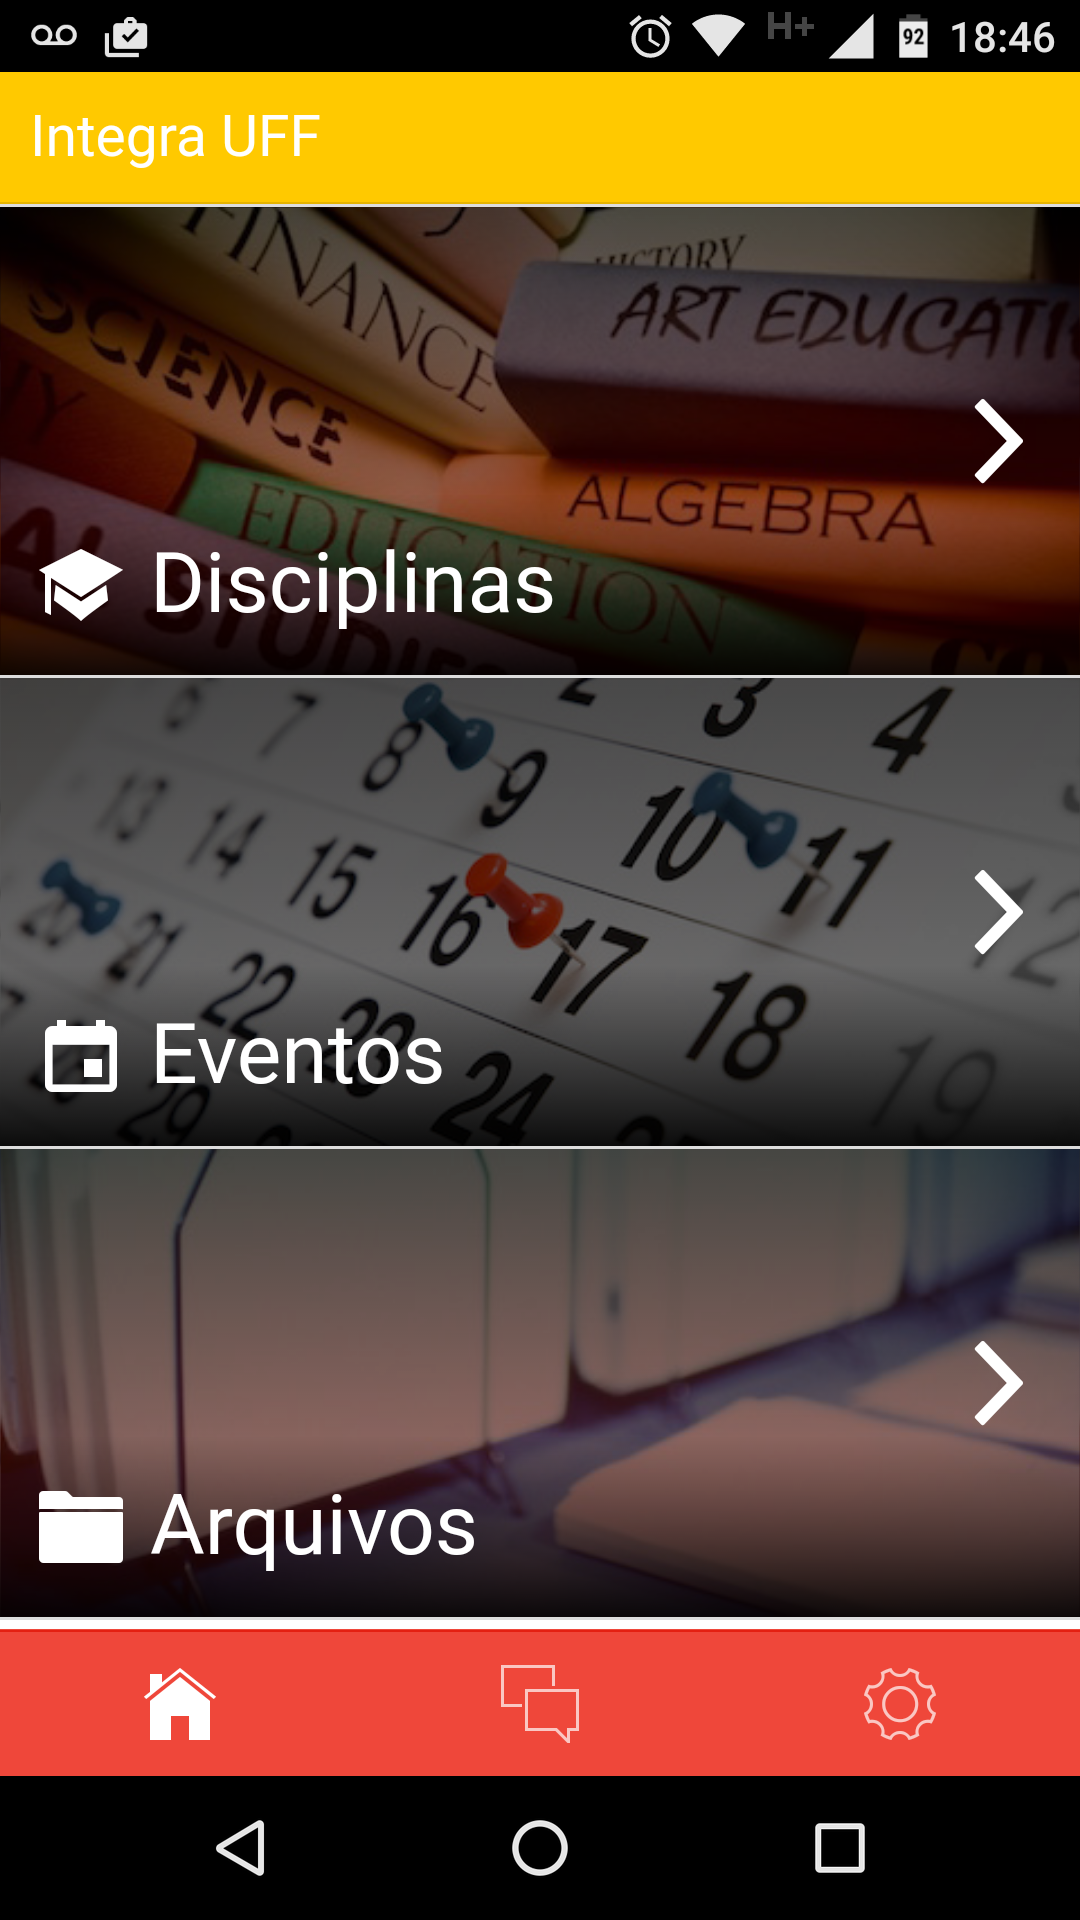
\includegraphics[scale=0.15]{menuprincipal}
    \caption{Menu do Integra UFF}
    \label{menuprincipal}
\end{figure}

\begin{table}[H]
  \begin{tabular}{ p{.20\textwidth} | p{.80\textwidth} }
    Trigger & O usuário acessa a aplicação\\
    \hline
    Pré condição & O usuário não sincronizou com nenhuma das aplicações anteriormente. O aparelho deve estar conectado à internet.\\
    \hline
    Caminho Básico &
    \begin{minipage}{5in}
      \vskip 4pt
      \begin{enumerate}
        \item O usuário escolhe a qual rede deseja se conectar selecionando com o toque na tela em um item dentre uma lista de opções.
        \item O sistema exibe um formulário de login com um campo para o e-mail e outro para a senha.
        \item O usuário preenche seus dados e seleciona sincronizar.
        \item O sistema sincroniza com a aplicação escolhida e exibe a tela principal com as opções Disciplinas, Eventos, Arquivos e Configurações.
      \end{enumerate}
      \vskip 4pt
    \end{minipage} \\
    \hline
    Caminho alternativo &
    \begin{minipage}{5in}
      \vskip 4pt
      Se o usuário já sincronizou com alguma aplicação anteriormente ele deve seguir os seguintes passos:
      \begin{enumerate}
        \item O usuário seleciona Configurações na tela principal.
        \item O usuário seleciona Contas Sincronizadas na tela de configurações.
        \item O sistema exibe a tela com as opções de aplicações disponíveis para sincronização.
        \item A partir daqui o usuário segue o caminho básico.
      \end{enumerate}
      \vskip 4pt
    \end{minipage} \\
    \hline
    Pós condição & Informações da aplicação sincronizada devem ser baixadas para o aparelho.\\
    \hline
    Caminho de exceção & O usuário pode abandonar a operação a qualquer momento. Caso o usuário erre o login o sistema deve exibir a tela de login informando o erro.
  \end{tabular}
  \caption{Sincronizar com uma aplicação}
  \label{table:sincronizacao}
\end{table}

\subsection{Acessar listagem de disciplinas}

As disciplinas representam o conteúdo principal da aplicação. Todos os outros conteúdos estão associados a ela. Portanto se fez necessário exibir uma listagem delas para o usuário, a qual é acessada pelo menu principal demonstrado anteriormente.

A listagem possui uma interface simples que informa o nome das disciplinas associadas e o semestre a qual ela pertence como mostra a figura \ref{indexdisciplinas}.

\begin{figure}[H]
    \centering
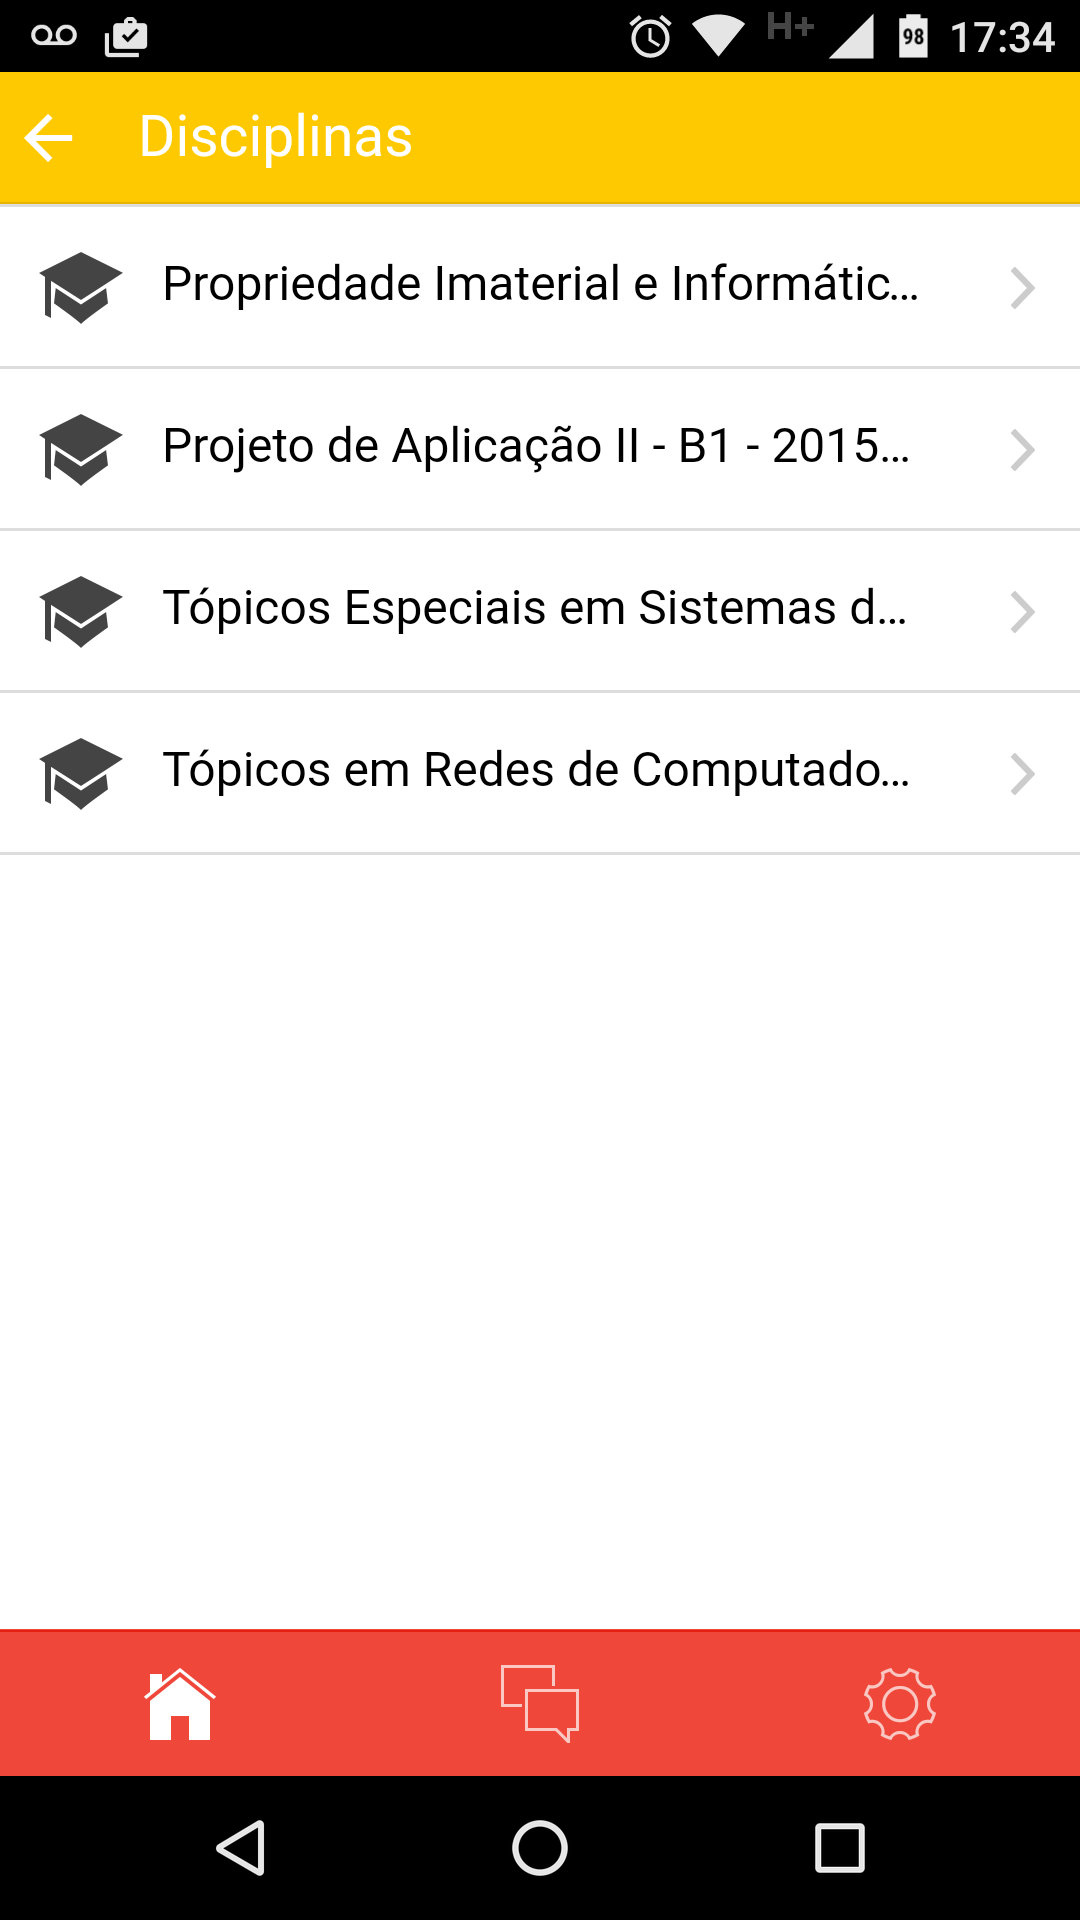
\includegraphics[scale=0.15]{indexdisciplinas}
    \caption{Listagem de Disciplinas}
    \label{indexdisciplinas}
\end{figure}

Ao clicar no nome de uma das disciplinas da lista, o usuário será redirecionado para uma seção contendo os detalhes da mesma.

O caso de uso desta funcionalidade é mostrado na tabela \ref{table:indexdisciplinas}.

\begin{table}[H]

  \begin{tabular}{ p{.20\textwidth} | p{.80\textwidth} }
    Trigger & O usuário acessa a aplicação.\\
    \hline
    Pré condição & O usuário está na tela do menu principal do sistema.\\
    \hline
    Caminho Básico &
    \begin{minipage}{5in}
      \vskip 4pt
      \begin{enumerate}
        \item O usuário seleciona a opção disciplinas no menu do sistema.
        \item O sistema exibe uma tela com uma lista de todas as disciplinas sincronizadas com o aparelho. A listagem contém o nome da disciplina.
      \end{enumerate}
      \vskip 4pt
    \end{minipage} \\
    \hline
    Caminho de exceção & O usuário pode abandonar a operação a qualquer momento.
 \end{tabular}
 \caption{Acessar listagem de disciplinas}
 \label{table:indexdisciplinas}
\end{table}

\subsection{Acessar detalhes de disciplinas}

Os detalhes de cada disciplina podem ser acessados através do clique em seu nome exibido na listagem. Nesta tela serão exibidas uma lista de tópicos, eventos e arquivos associados àquela disciplina, conforme a figura \ref{showdisciplina}, viabilizando uma forma simples de visualizar todos os conteúdos de uma disciplina específica.

\begin{figure}[H]
    \centering
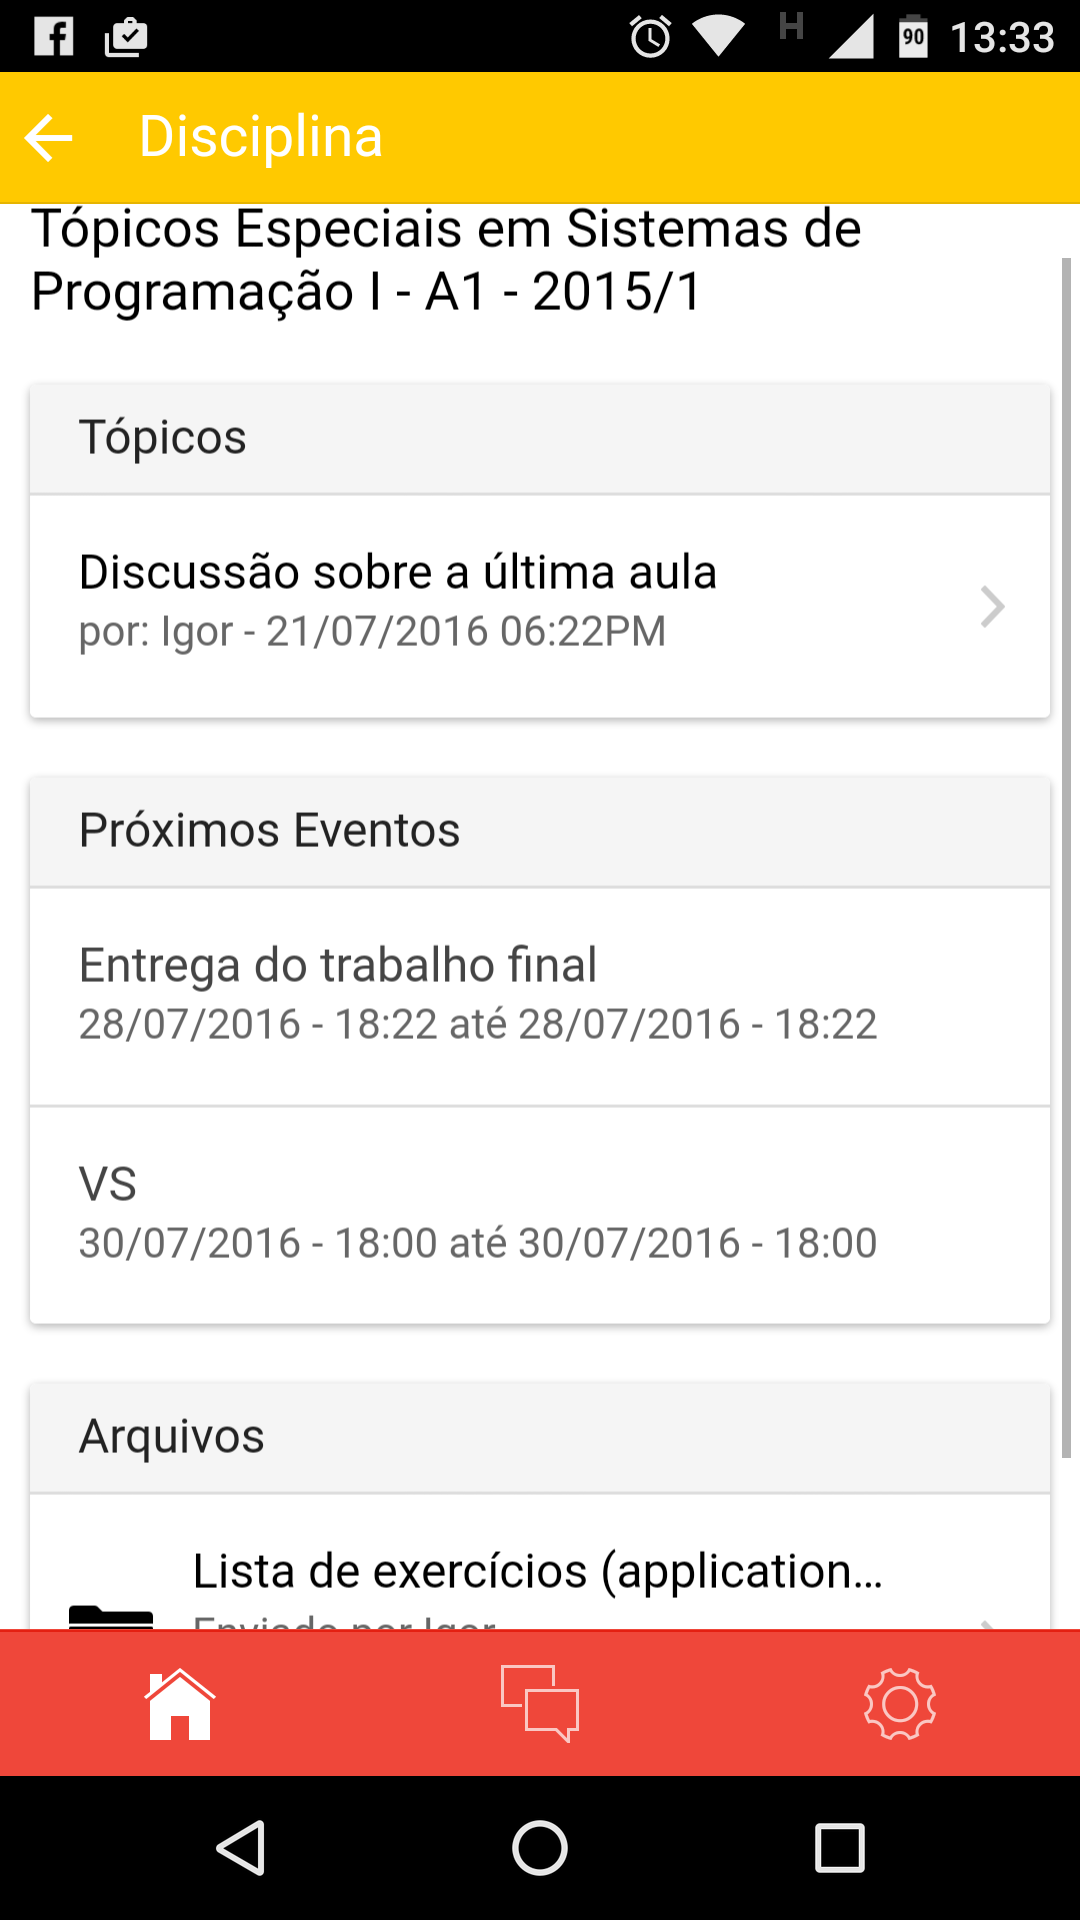
\includegraphics[scale=0.15]{showdisciplina}
    \caption{Detalhes de uma Disciplina}
    \label{showdisciplina}
\end{figure}

O clique no nome de um arquivo ou tópico redireciona o usuário para a página de detalhes dos mesmos.

O caso de uso desta funcionalidade é mostrado na tabela \ref{table:showdisciplina}.

\begin{table}[H]
  \begin{tabular}{ p{.20\textwidth} | p{.80\textwidth} }
    Trigger & O usuário acessou a tela de listagem de disciplinas.\\
    \hline
    Pré condição & O usuário possui alguma disciplina sincronizada com o aparelho.\\
    \hline
    Caminho Básico &
    \begin{minipage}{5in}
      \vskip 4pt
      \begin{enumerate}
        \item O usuário seleciona uma das disciplinas da listagem.
        \item O sitema exibe uma tela contendo as seguintes informações sobre a disciplina: nome, últimos tópicos, próximos eventos e últimos arquivos.
      \end{enumerate}
      \vskip 4pt
    \end{minipage} \\
    \hline
    Caminho de exceção & O usuário pode abandonar a operação a qualquer momento.
  \end{tabular}
  \caption{Acessar detalhes de disciplinas}
  \label{table:showdisciplina}
\end{table}

\subsection{Acessar listagem de arquivos}

Apesar de ser possível acessar a lista de arquivos de uma disciplina na tela de listagem da última, também está disponível uma listagem de arquivos sincronizados através do clique na opção Arquivos no menu principal da aplicação. Esta listagem demonstra todos os arquivos sicronizados, agrupados pelas disciplinas a qual pertencem, como mostra a figura \ref{indexarquivos}

\begin{figure}[H]
    \centering
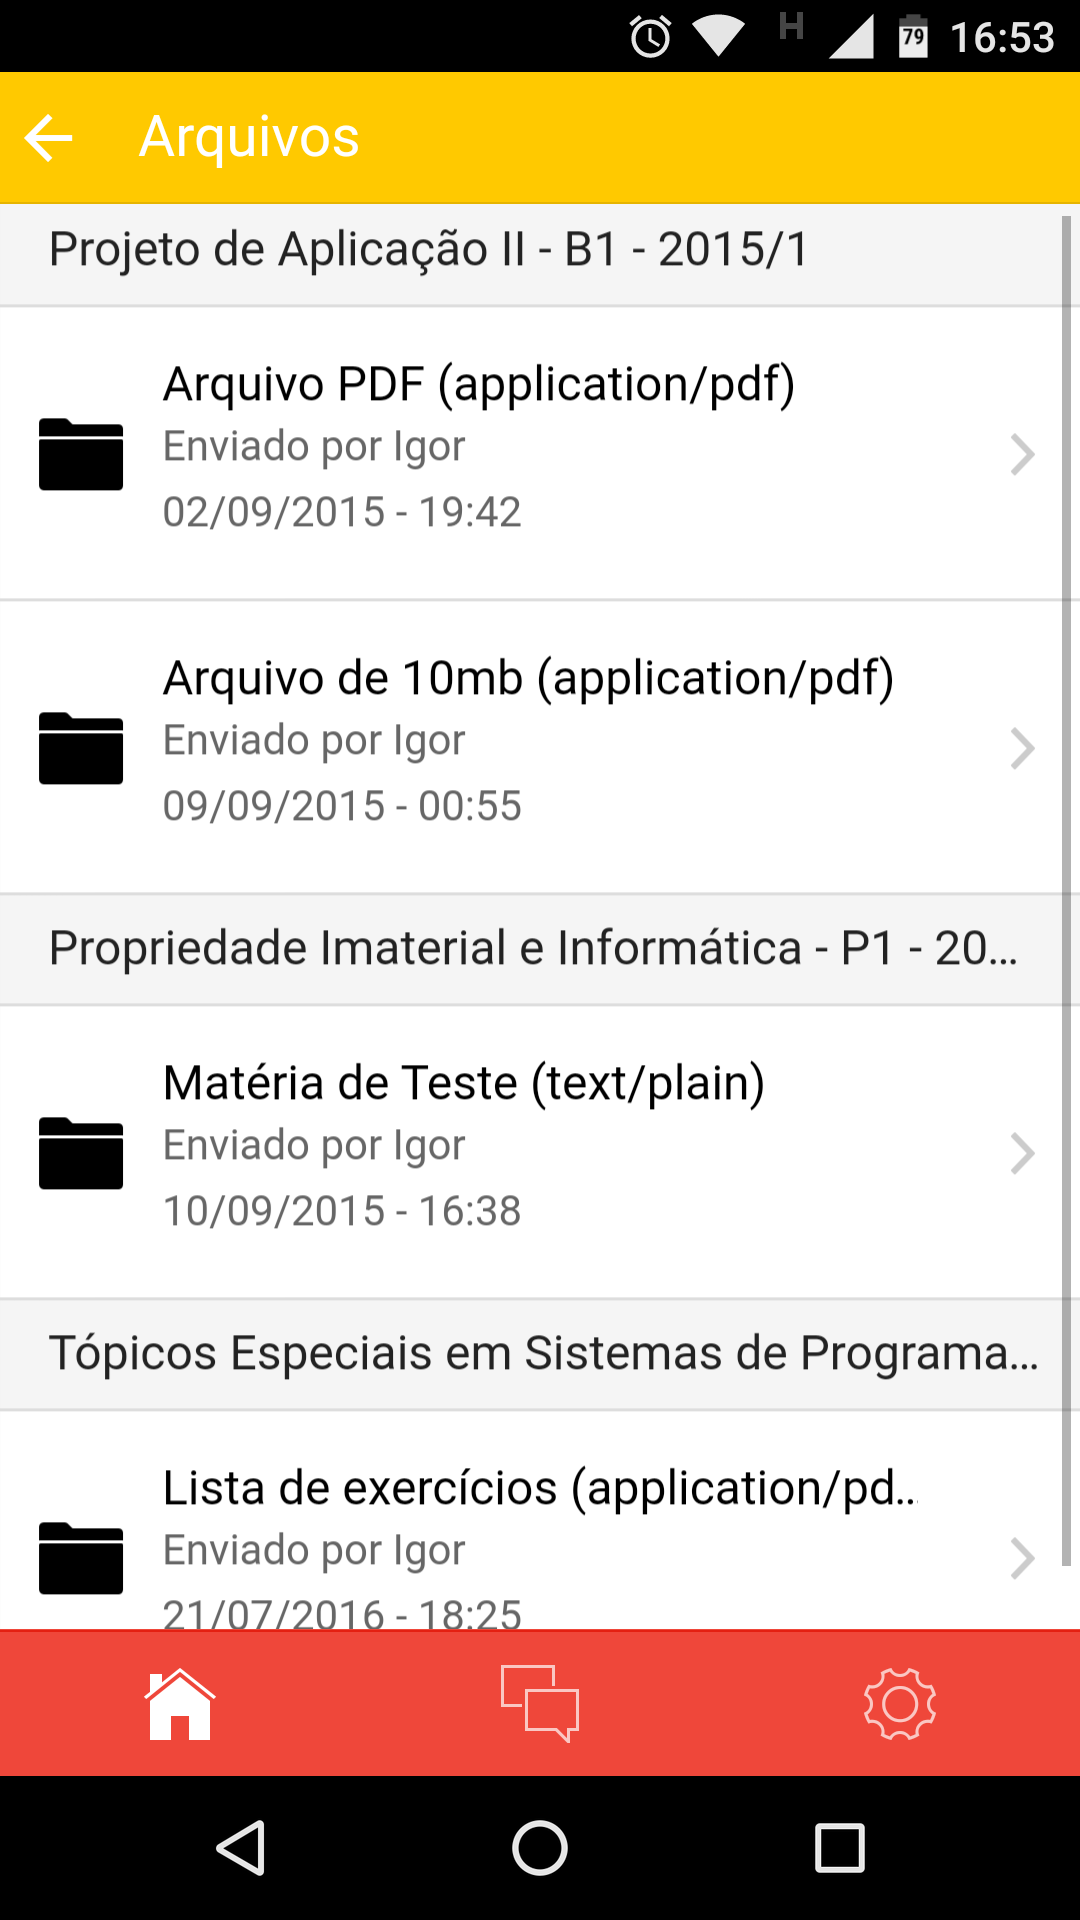
\includegraphics[scale=0.15]{indexarquivos}
    \caption{Listagem de Arquivos}
    \label{indexarquivos}
\end{figure}

Clicando em qualquer um dos arquivos o usuário será redirecionado para a página de detalhes deste. A tabela \ref{table:indexarquivos} apresenta o caso de uso desta funcionalidade.

\begin{table}[H]
  \begin{tabular}{ p{.20\textwidth} | p{.80\textwidth} }
    Trigger & O usuário acessa a aplicação.\\
    \hline
    Pré condição & O usuário possui alguma disciplina sincronizada com o aparelho.\\
    \hline
    Caminho Básico &
    \begin{minipage}{5in}
      \vskip 4pt
      \begin{enumerate}
        \item O usuário seleciona a opção arquivos no menu do sistema.
        \item O sistema exibe uma tela com uma lista de todos os arquivos sincronizados com o aparelho. A listagem contém as seguintes informações dos arquivos: nome, formato, quem o enviou, data e hora de envio. Os arquivos exibidos são organizados por disciplinas.
      \end{enumerate}
      \vskip 4pt
    \end{minipage} \\
    \hline
    Caminho de exceção & O usuário pode abandonar a operação a qualquer momento.
  \end{tabular}
  \caption{Acessar listagem de arquivos}
  \label{table:indexarquivos}
\end{table}

\subsection{Acessar detalhes de arquivos}

Conforme as citações anteriores a página de detalhes de arquivos pode ser acessada através da listagem geral de arquivos, ou da listagem de arquivos na tela de detalhes de uma disciplina. Esta tela contém o nome do arquivo e informações do formato, tamanho, data e hora em que foi enviado e o nome de quem o enviou, visto na figura \ref{showarquivo}. Além de possuir um botão para realizar o \textit{download} para o dispositivo.  

\begin{figure}[H]
    \centering
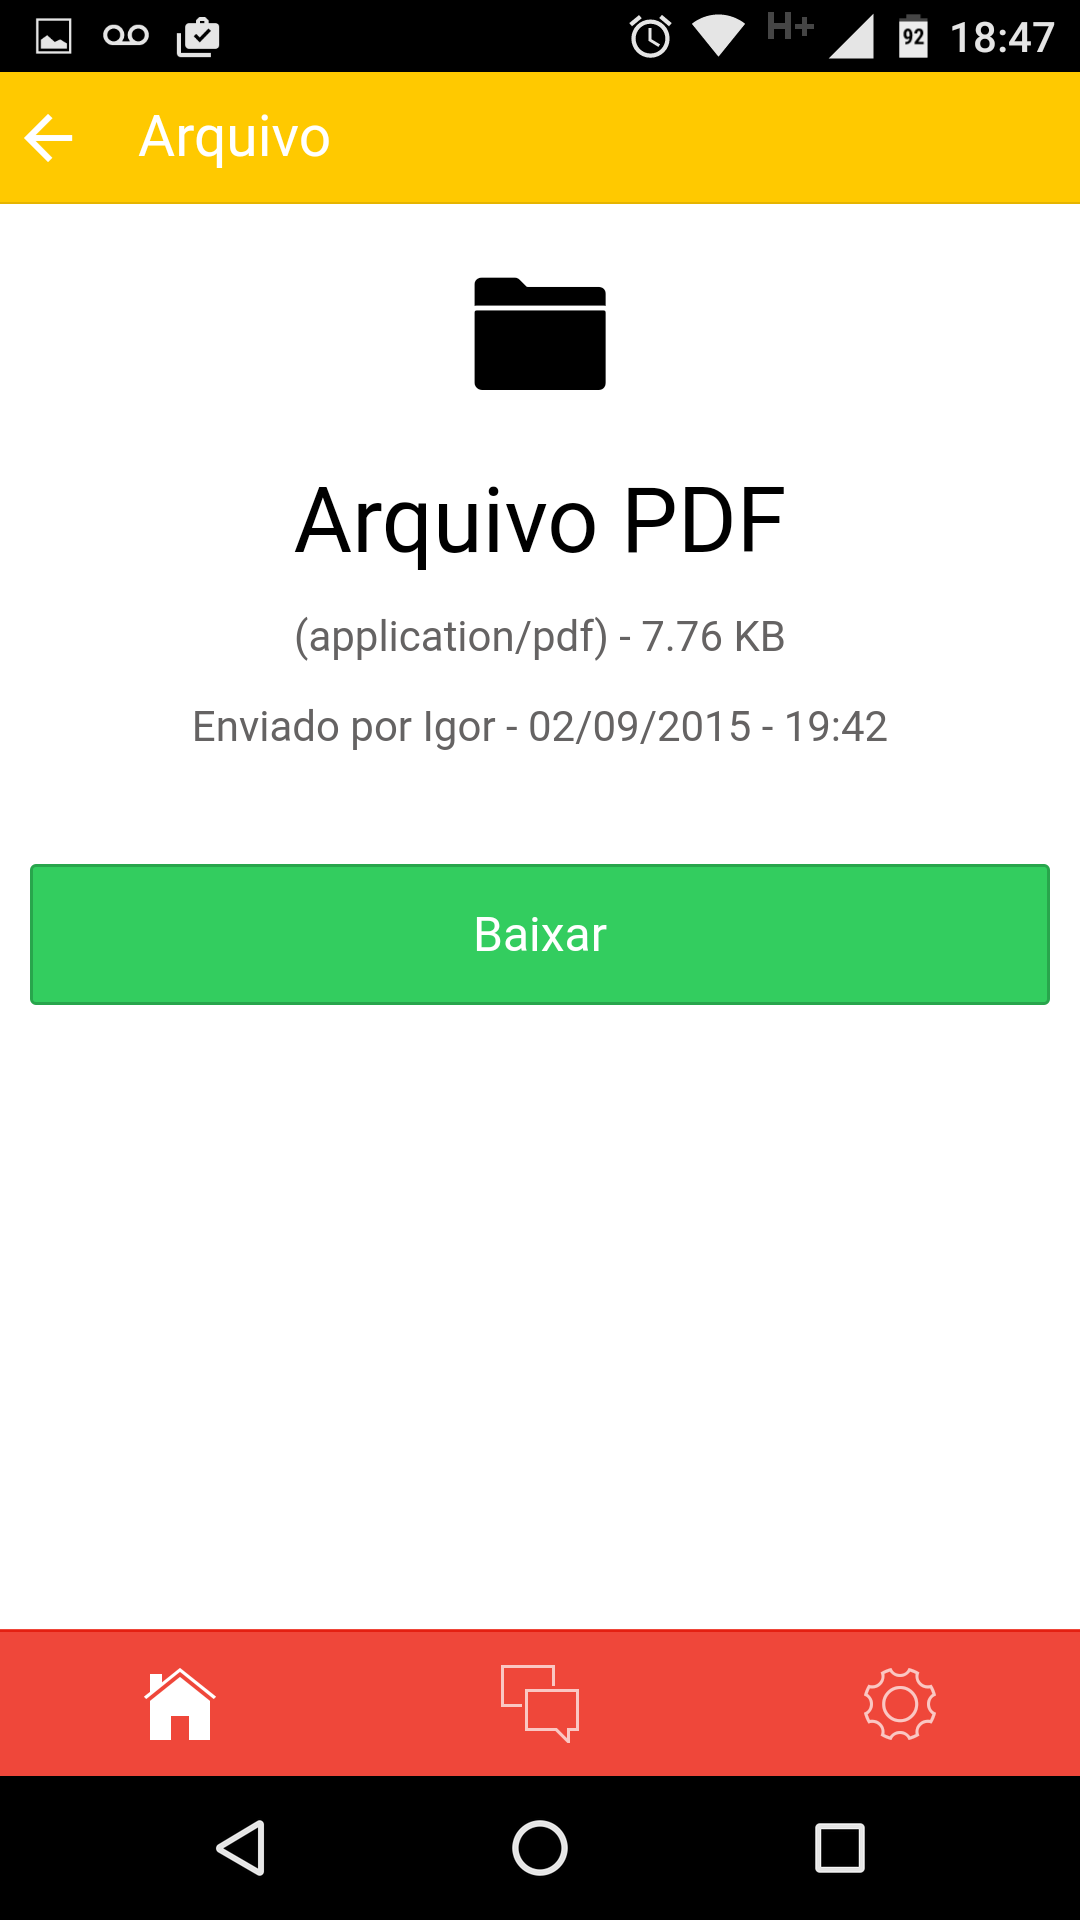
\includegraphics[scale=0.15]{showarquivo}
    \caption{Detalhes de um Arquivo}
    \label{showarquivo}
\end{figure}

Caso o arquivo já tenha sido baixado, a tela irá exibir um botão para abri-lo e um \textit{link} para apagá-lo.

A tabela \ref{table:showarquivo} evidencia o caso de uso.

\begin{table}[H]
  \begin{tabular}{ p{.20\textwidth} | p{.80\textwidth} }
    Trigger & O usuário acessou a tela de listagem de arquivos.\\
    \hline
    Pré condição & O usuário possui algum arquivo sincronizado com o aparelho.\\
    \hline
    Caminho Básico &
    \begin{minipage}{5in}
      \vskip 4pt
      \begin{enumerate}
        \item O usuário seleciona um dos arquivos da listagem.
        \item O sitema exibe uma tela contendo as seguintes informações sobre o arquivo: nome, formato, tamanho, quem o enviou, data e hora do envio, um botão para baixá-lo.
      \end{enumerate}
      \vskip 4pt
    \end{minipage} \\
    \hline
    Caminho de exceção & O usuário pode abandonar a operação a qualquer momento.
  \end{tabular}
  \caption{Acessar detalhes de arquivos}
  \label{table:showarquivo}
\end{table}

\subsection{Baixar arquivos}

Baixar os arquivos é possível através de um botão na tela de detalhes de um arquivo. O procedimento é demonstrado pela figura \ref{downloadarquivo} e o caso de uso pela tabela \ref{table:downloadarquivo}.

\begin{figure}[H]
    \centering
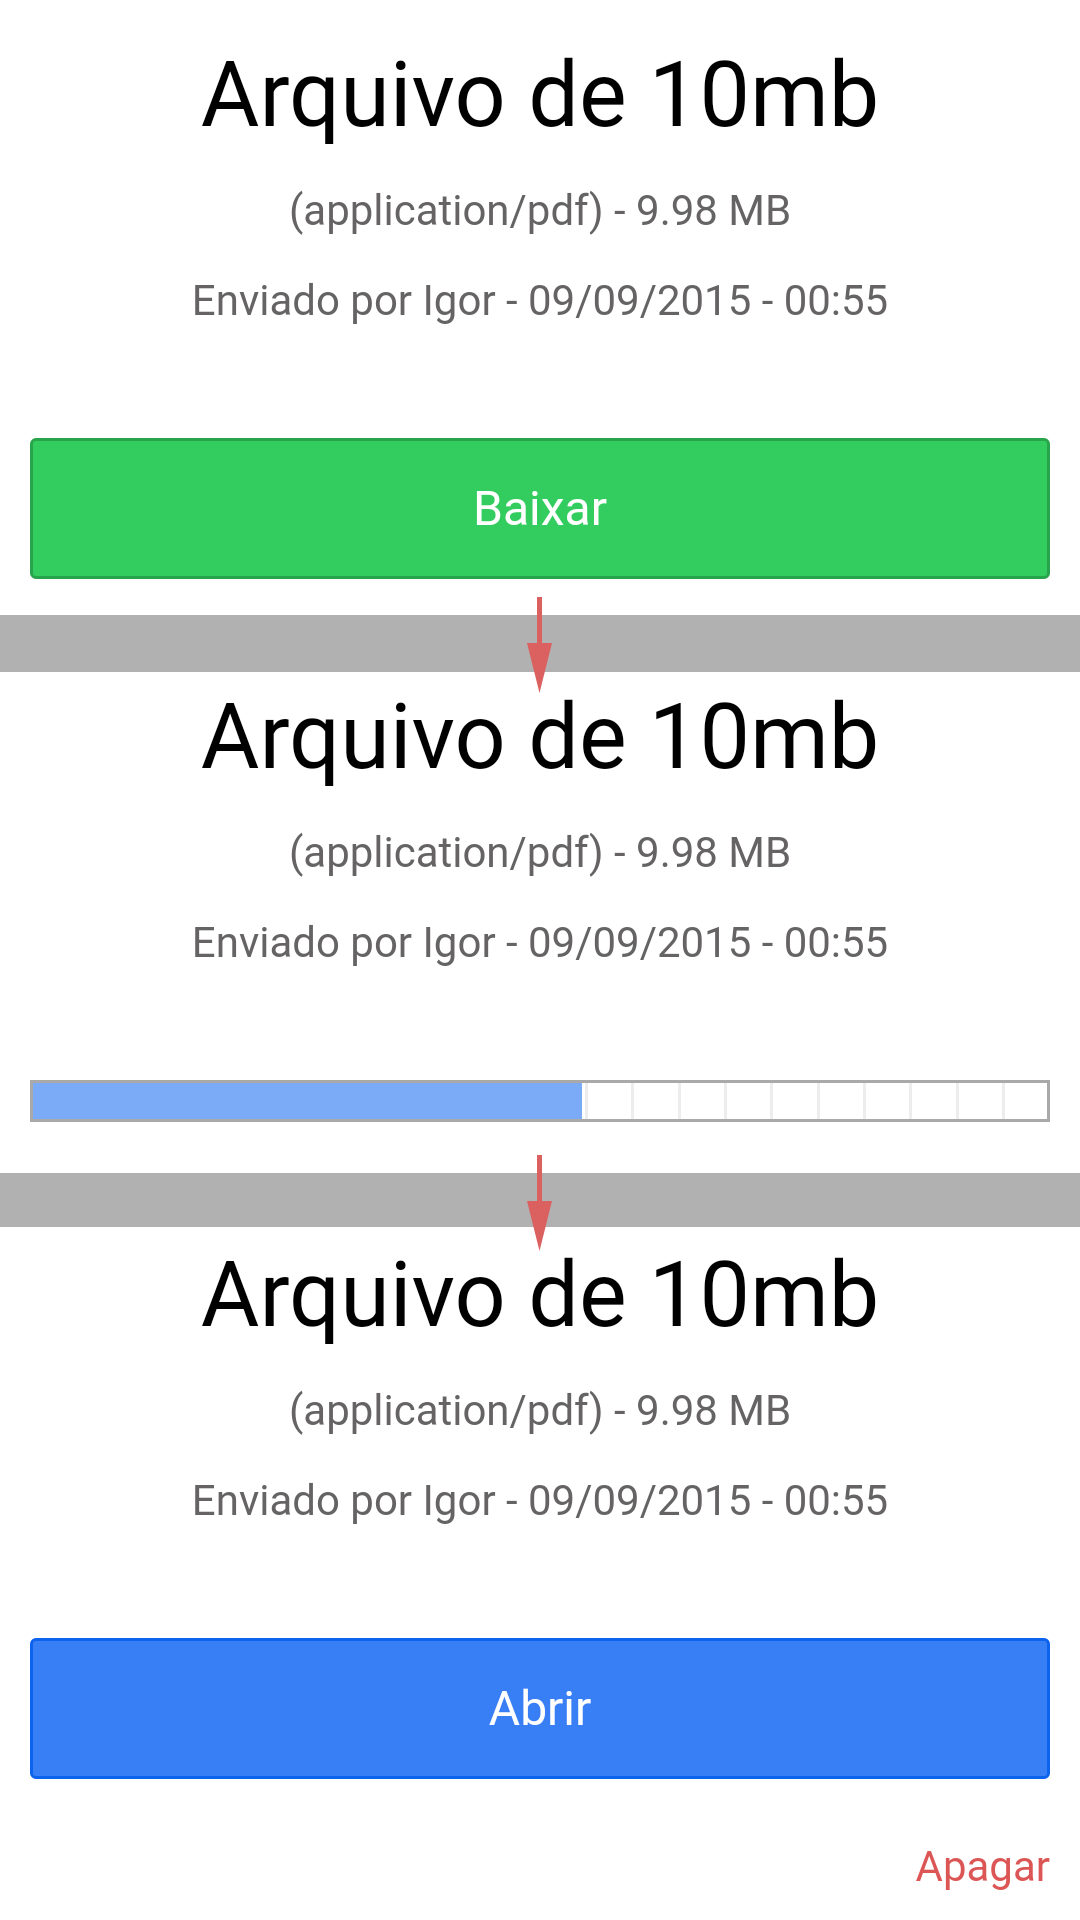
\includegraphics[scale=0.15]{downloadarquivo}
    \caption{\textit{Download} de um Arquivo}
    \label{downloadarquivo}
\end{figure}

\begin{table}[H]
  \begin{tabular}{ p{.20\textwidth} | p{.80\textwidth} }
    Trigger & O usuário acessa a página de detalhes de um arquivo.\\
    \hline
    Pré condição & O usuário possui algum arquivo sincronizado com o aparelho. O aparelho deve estar conectado à internet.\\
    \hline
    Caminho Básico &
    \begin{minipage}{5in}
      \vskip 4pt
      \begin{enumerate}
        \item O usuário aperta o botão download.
        \item O sistema inicia o download do arquivo selecionado.
      \end{enumerate}
      \vskip 4pt
    \end{minipage} \\
    \hline
    Pós condição & O arquivo selecionado deve ser baixado para o aparelho do usuário e o sistema deve mostrar os botões para abrir e apagar o arquivo.\\
    \hline
    Caminho de exceção & O usuário pode abandonar a operação a qualquer momento.\\
    \hline
  \end{tabular}
  \caption{Baixar arquivos}
  \label{table:downloadarquivo}
\end{table}

\subsection{Apagar arquivos}

Apagar os arquivos, assim como o seu \textit{download}, é realizado através de um \textit{link} na tela de detalhes de um arquivo. O procedimento é demonstrado pela figura \ref{apagararquivo} e o caso de uso pela tabela \ref{table:apagararquivo}.

\begin{figure}[H]
    \centering
\includegraphics[scale=0.15]{apagararquivo}
    \caption{Apagar um Arquivo}
    \label{apagararquivo}
\end{figure}


\begin{table}[H]
  \begin{tabular}{ p{.20\textwidth} | p{.80\textwidth} }
    Trigger & O usuário acessa a página de detalhes de um arquivo.\\
    \hline
    Pré condição & O usuário possui algum arquivo baixado no aparelho.\\
    \hline
    Caminho Básico &
    \begin{minipage}{5in}
      \vskip 4pt
      \begin{enumerate}
        \item O usuário aperta o botão apagar.
      \end{enumerate}
      \vskip 4pt
    \end{minipage} \\
    \hline
    Pós condição & O arquivo selecionado deve ser apagado do aparelho do usuário e o sistema deve exibir o botão para baixar o arquivo.\\
    \hline
    Caminho de exceção & O usuário pode abandonar a operação a qualquer momento.\\
    \hline
  \end{tabular}
  \caption{Apagar arquivos}
  \label{table:apagararquivo}
\end{table}

\subsection{Acessar listagem de eventos}

A listagem de eventos reúne todos os eventos sincronizados no dispositivo. Os eventos são agrupados por próximos, eventos prestes a acontecerem, e encerrados como mostra a figura \ref{indexeventos}. Esta listagem também informa a qual disciplina cada evento pertence.

\begin{figure}[H]
    \centering
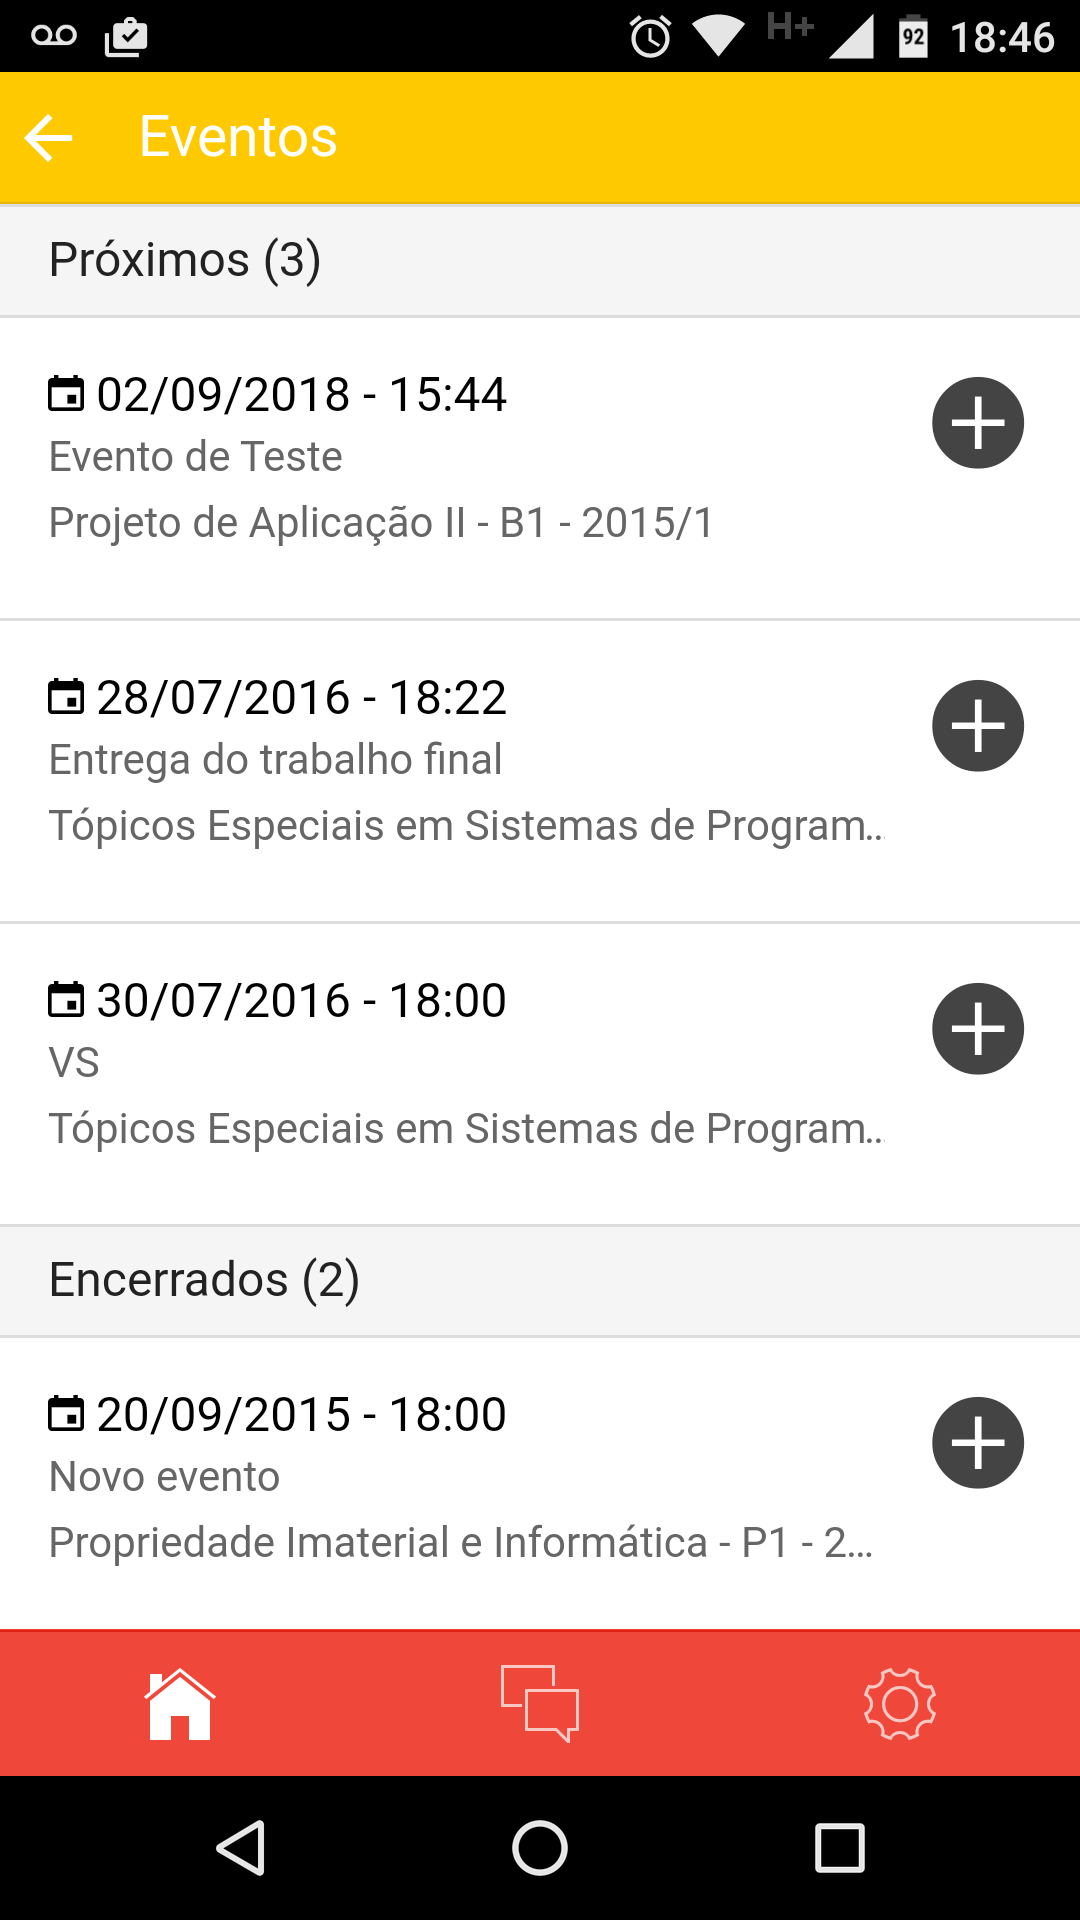
\includegraphics[scale=0.15]{indexeventos}
    \caption{Listagem de Eventos}
    \label{indexeventos}
\end{figure}

O caso de uso pode ser observado na tabela \ref{table:indexeventos}.

\begin{table}[H]
  \begin{tabular}{ p{.20\textwidth} | p{.80\textwidth} }
    Trigger & O usuário acessa a aplicação.\\
    \hline
    Pré condição & O usuário está na tela do menu principal do sistema.\\
    \hline
    Caminho Básico &
    \begin{minipage}{5in}
      \vskip 4pt
      \begin{enumerate}
        \item O usuário seleciona a opção eventos no menu do sistema.
        \item O sistema exibe uma tela com uma lista de todos os eventos sincronizados com o aparelho. A listagem contém as seguintes informações dos eventos: nome, data, hora e disciplina. Os eventos são exibidos separadamente entre próximos eventos e eventos passados.
      \end{enumerate}
      \vskip 4pt
    \end{minipage} \\
    \hline
    Caminho de exceção & O usuário pode abandonar a operação a qualquer momento.\\
    \hline
  \end{tabular}
  \caption{Acessar listagem de eventos}
  \label{table:indexeventos}
\end{table}

\subsection{Adicionar evento ao calendário}

Os eventos podem ser adicionados no calendário padrão do dispositivo utilizado pelo usuário. Para isso é preciso acessar a listagem dos eventos e clicar no ícone ao lado direito do evento escolhido. Uma caixa de diálogo será exibida confirmando a operação. A figura \ref{addevento} ilustra o procedimento, e o caso de uso é descrito pela tabela \ref{table:addevento}.

\begin{figure}[H]
    \centering
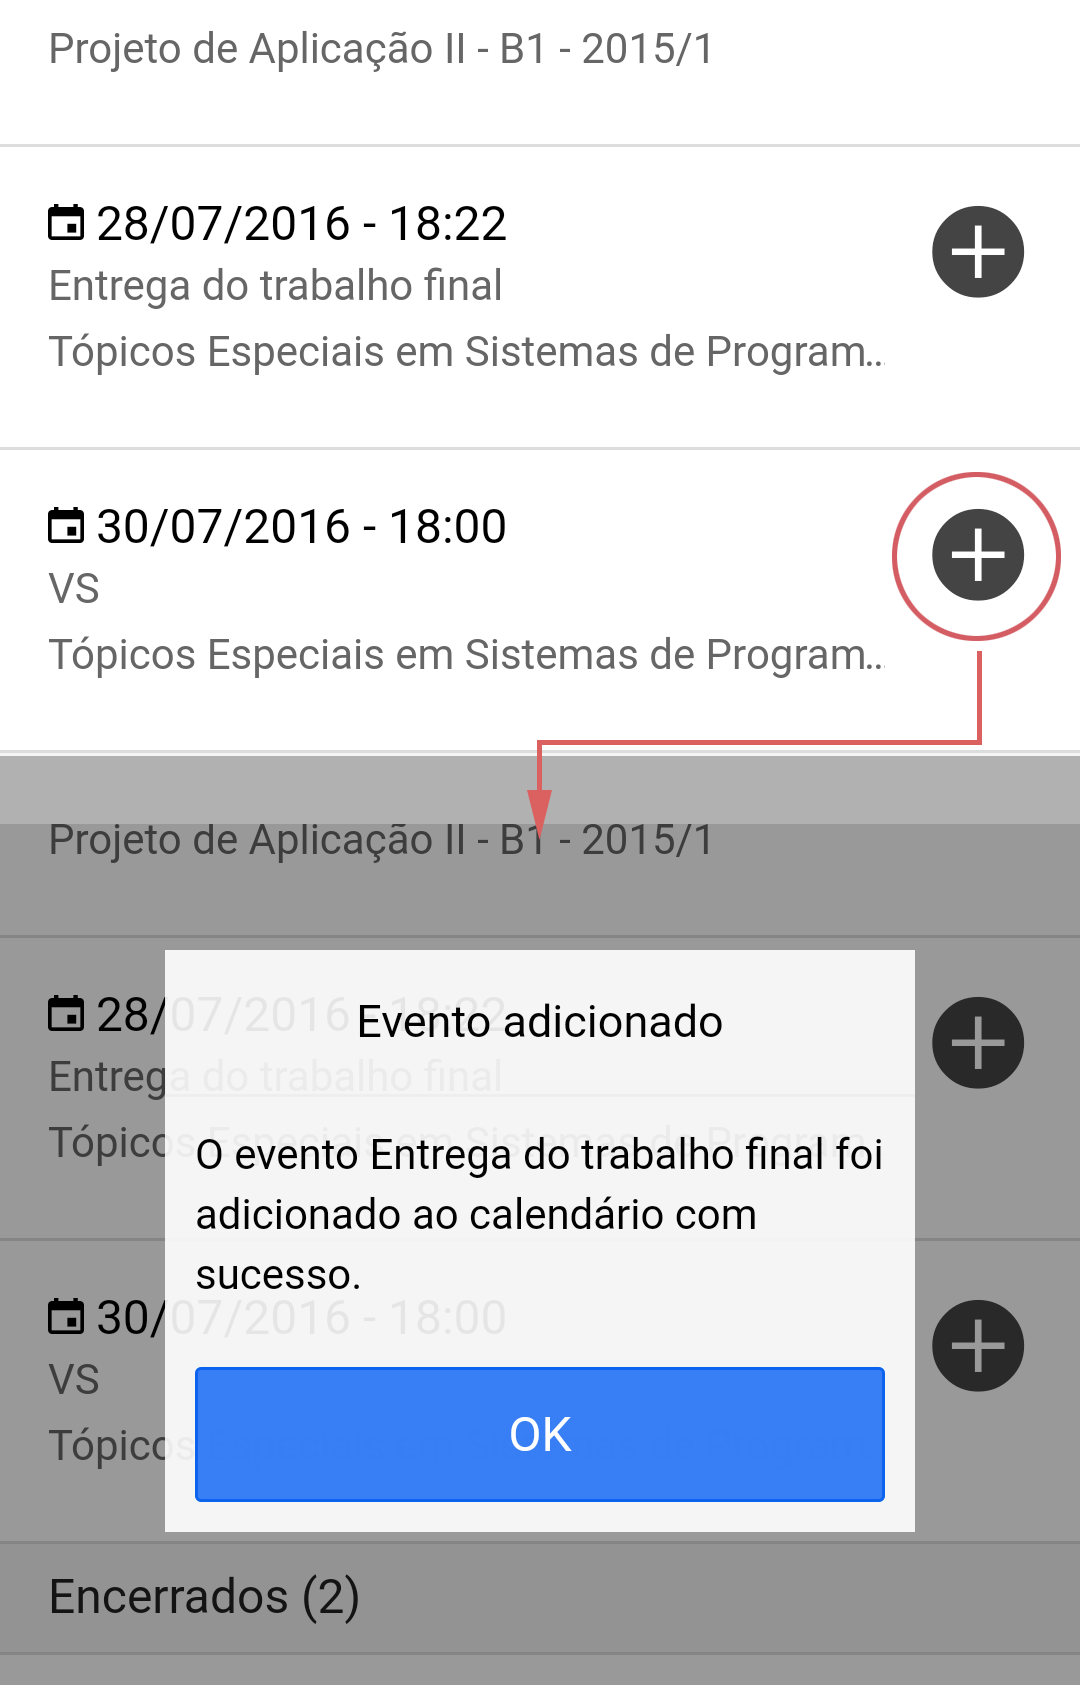
\includegraphics[scale=0.15]{addevento}
    \caption{Adicionar evento ao calendário}
    \label{addevento}
\end{figure}

\begin{table}[H]
  \begin{tabular}{ p{.20\textwidth} | p{.80\textwidth} }
    Trigger & O usuário acessa a página de listagem de eventos.\\
    \hline
    Pré condição & O usuário possui algum evento sincronizado no aparelho.\\
    \hline
    Caminho Básico &
    \begin{minipage}{5in}
      \vskip 4pt
      \begin{enumerate}
        \item O usuário seleciona o ícone de adicionar situado ao lado do evento que deseja colocar no calendário.
      \end{enumerate}
      \vskip 4pt
    \end{minipage} \\
    \hline
    Pós condição & O evento selecionado deve ser criado no calendário nativo do aparelho do usuário.\\
    \hline
    Caminho de exceção & O usuário pode abandonar a operação a qualquer momento.\\
    \hline
  \end{tabular}
  \caption{Adicionar evento ao calendário}
  \label{table:addevento}
\end{table}

\section{Outros requisitos não funcionais}

\subsection{Requisitos de segurança}

Para a utilização do sistema o usuário precisará sincronizar a aplicação com as plataformas disponíveis. Para tal será necessário uma autenticação, esta será feita pelas próprias plataformas integradas ao sistema.

\subsection{Atributos de Qualidade de Software}

O sistema precisa possuir uma arquitetura que permita uma fácil extensão através do desenvolvimento de plugins. Também deve possuir o código aberto e contar com testes automatizados que garantem que os requisitos sejam atendidos e continuem funcionando a cada nova contribuição ao código fonte. Métricas devem ser rodadas a cada nova revisão para que a qualidade final do produto seja mantida.
